
\documentclass{article}

\usepackage{a4wide,tikz}
\usetikzlibrary{mindmap,trees}
\usepackage[margin=0pt,hmargin={-0.5cm,0cm},papersize={16.9cm,12cm}]{geometry} 
\begin{document}
\pagestyle{empty}


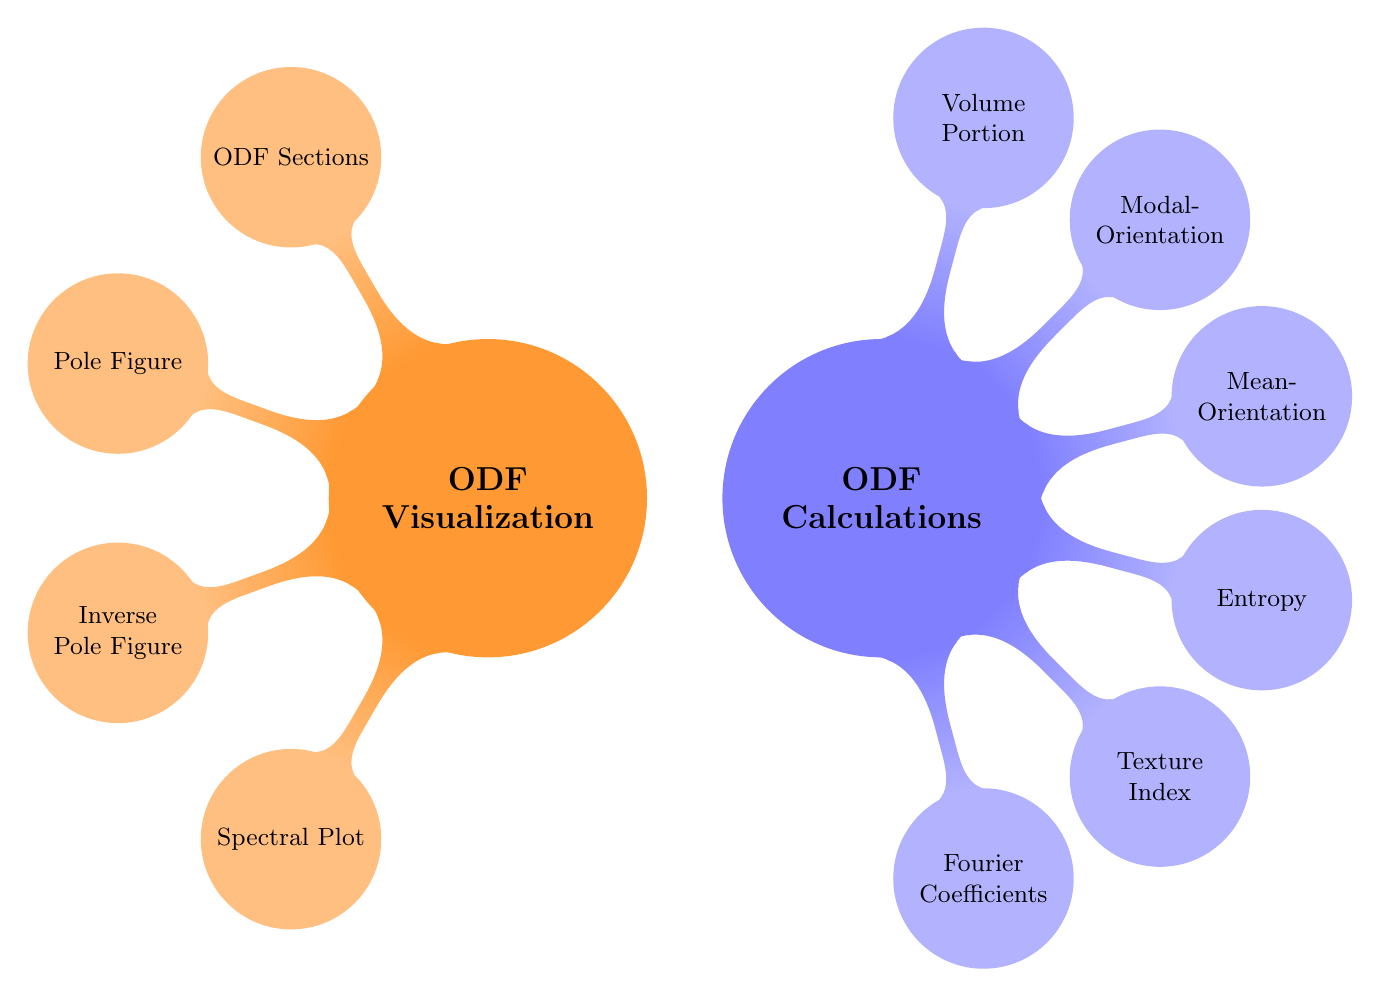
\begin{tikzpicture}[scale = 1]
  \definecolor{myblue}{HTML}{92dcec}
  \tikzstyle{every annotation}=[fill=white, font=\sf]

  \path[mindmap, concept color=orange!80!]
  node[concept] {\bf ODF\\ Visualization} 
  child[grow = 120, concept color=orange!50] 
  { node(ebsd) [concept](ebsd2) {ODF Sections}}
  child[grow = 160, concept color=orange!50] 
  { node[concept](pf) {Pole Figure}}
  child[grow = -160, concept color=orange!50] 
  { node[concept](pf) {Inverse Pole Figure}}
  child[grow = -120, concept color=orange!50] 
  { node[concept](pf) {Spectral Plot}};

  \path[mindmap, concept color=blue!50!]
  node[concept] at (5,0){\bf ODF \\Calculations} 
  child[grow=75, concept color=blue!30] 
  { node(ebsd) [concept](ebsd2) {Volume Portion}}
  child[grow=45, concept color=blue!30] 
  { node[concept](pf) {Modal\-Orientation}}
  child[grow=15, concept color=blue!30] 
  { node[concept](pf) {Mean\-Orientation}}
  child[grow=-15, concept color=blue!30] 
  { node[concept](pf) {Entropy}}
  child[grow=-45, concept color=blue!30] 
  { node[concept](pf) {Texture Index}}
  child[grow=-75, concept color=blue!30] 
  { node[concept](pf) {Fourier Coefficients}};

\end{tikzpicture}
\end{document}
%%% Local Variables: 
%%% mode: latex
%%% TeX-master: t
%%% End: 
